\chapter{Facial Recognition}\label{ch:face-rec}
Facial recognition is a task of verifying or identifying a person from digital image/video.

As I mentioned in the definition, there are two main subtasks~\cite{FaceRec}:
\begin{enumerate}
    \item \textbf{Verification} deals with verifying whether the person in the image is who he claims he is.
    A typical modern use case of verification is smartphone unlocking with face.
    An example of such system is Face ID developed by Apple Inc.

    \item \textbf{Identification} is a task of matching a person to an identity.
    To formulate it in another way, the goal of identification is to give us an answer to the question of who the person
    in the image is.
\end{enumerate}

\section{Pipeline}\label{sec:pipeline}
Facial recognition pipeline\footnote{\label{foot:pipe}A chain of processing elements, arranged so that the output of
each element is the input of the next.} usually has the following four steps:
\begin{enumerate}
    \item The first one is \textbf{face detection}.
    As the name implies it deals with determination of face location within the image.
    The output of the algorithm is usually face coordinates and facial landmarks.
    Landmarks are a set of coordinates marking important points of the face (eyebrows, nose, mouth, \ldots).
    The knowledge of these points is a necessity for the following step.
    An example of face detection system is described in section~\ref{sec:face-detection}.
    \item \textbf{Face alignment} is a task of changing the face position in such a way that it resembles the position
    of faces on which the feature extraction model was trained.
    In most of the instances this step improves the accuracy.
    \item \textbf{Feature extraction} is a process of computing a feature vector\footnote{A feature vector is a vector
    that contains information describing an object's important characteristics.} of the face.
    Architecture of models used for feature extraction was described in the previous chapter~\ref{ch:cnn}.
    \item \textbf{Feature matching} uses feature vector from the previous task to identify a person in the image.
    The algorithm uses a database of pre-computed feature vectors and compares them to the newly extracted one.
    The identity associated with the feature vector which has the smallest distance from the extracted one is
    considered to be the identity of the person in the image.
\end{enumerate}

It is important to note that the second step is not always present and it is deemed unnecessary by some~\cite{FaceNet}.

\section{Datasets}\label{sec:datasets}
In this section I will briefly describe datasets used for training and evaluation of facial recognition models.
There are too many different datasets used in practice.
For this reason I will focus only on those mentioned in this text.

\subsection{LFW}\label{subsec:lfw}
LFW is an acronym for Labeled Faces in the Wild.
The dataset contains 13,000 images and 1680 identities.
Every identity is represented by at least two samples.
The faces were detected by Viola-Jones face detector\footnote{Real-time object detection framework.}.

There are now four publicly used versions of the dataset.
These versions are differentiated by the type of preprocessing (different methods of alignment) applied to the images.

\subsection{YTF}\label{subsec:ytf}
YTF stands for YouTube Faces.
The data set contains 3425 videos and 1,595 unique identities.
The average length of the video clip is 181.3 frames and there are on average 2.15 videos for each subject.

\subsection{MS-Celeb-1M}\label{subsec:ms1m}
MS-Celeb-1M is a dataset constructed by Microsoft Research.
There are 10 million face images with nearly 100,000 individuals.
The data were harvested from the Internet.

Due to the method with which the images were collected there are many mislabellings in the dataset.
For this reason there are different versions available on the Internet containing refined data (like MS1MV2).

As the name implies the dataset contains images of celebrities.
In this context celebrity is assumed to be anyone with frequent online presence.
This became a controversial issue and as a result Microsoft pulled the dataset off the internet.

\section{Face Detection}\label{sec:face-detection}
As I mentioned in the description of a facial recognition pipeline the goal of face detection is to find the location
of the face within the image.
This is challenging in unconstrained environments due to various poses, illuminations and occlusions.

To not digress too much from the main topic I will describe only the system which was put in use in the experimental
part of this thesis.
The detection algorithm is called MTCNN~\ref{subsec:mtcnn}.

Before going through the process of face detection it is necessary to describe a method called Non-maximum Suppression.

\subsection{Non-maximum Suppression}\label{subsec:nms}
Non-maximum Suppression (NMS) is a filtering algorithm of overlapping bounding
boxes\footnote{\label{foot:bbox}A rectangle describing face position.}.
NMS consists of five simple steps:
\begin{enumerate}
    \item \label{itm:nmss1}Create a list of proposal bounding boxes ordered by the confidence score.
    \item Select the bounding box with highest confidence score and add it to the filtered list of boxes.
    \item Compute IoU~\ref{fig:iou} between the selected bounding box and all the remaining ones.
    \item Remove all the boxes whose IoU is higher than some predetermined threshold.
    \item Go to~\ref{itm:nmss1} and repeat the process until there are no remaining bounding boxes within the original list.
\end{enumerate}

Having NMS defined we can proceed with actual face detection.

\subsection{MTCNN}\label{subsec:mtcnn}
MTCNN~\cite{MTCNN} stands for Multi-task Cascaded Convolutional Networks.
This model consists of three stages.

\subsubsection{Stage 1}
The first stage is called \textbf{Proposal Network} (P-Net) and its role is to find the candidate windows and their
bounding box regression vectors.
P-Net is fully convolutional neural network.

Before passing the image to P-Net we resize the image to many different sizes.
By doing so we make the model scale invariant.

Now we feed the images to the net.

The net produces many bounding boxes with a varying confidence.
We parse the output and delete the boxes with low confidence score.

Now we standardize the coordinates by converting the boxes from the coordinate systems of the resized images to
that of the unscaled one.

At this point we run NMS~\ref{subsec:nms} once for every scaled image.
Then we put all the survivors into one list and run NMS once more.

Before passing the boxes to stage 2 we make the boxes square by elongating the shorter sides.

\subsubsection{Stage 2}
The name of the second stage is \textbf{Refined Network} (R-Net).
The purpose of this stage is to filter out a large number of false positives and to calibrate the boxes.

Initially we take the boxes from the previous stage and copy the pixel values to separate arrays.
In case the box is out of bounds we fill the "empty space" with zeros.

Now we resize all the arrays to have the size of $24 \times 24$ pixels.
Currently the pixel values are in the range of $<0; 255>$ which is not optimal for the model training.
To work around the issue we normalize the values to $<-1; 1>$.

At this point we feed the images to R-Net and collect the outputs.

The outputs are similar to that of P-Net.
They also include the coordinates and the confidence levels.
The difference is that the new coordinates are more accurate.

In the last few steps of the stage 2 we remove the boxes with a lower confidence and perform NMS to remove the
redundant ones.

Now we standardize the coordinates and reshape the bounding boxes to a square.

\subsubsection{Stage 3}
In the last stage we take the boxes from stage 2 and copy the pixel values to separate arrays.
If there are any boxes which cross the image bounds we deal with then in the same way as in the previous stage.
That is we fill the empty space with zeros.

Now we resize the images to be of $48 \times 48$ pixels and feed them into a neural network called
\textbf{The Output Network} (O-Net).

O-Net is split into three layers at the top and as a result of this architectural choice produces three outputs:
the coordinates of the bounding box, the coordinates of the facial landmarks and the confidence level of each box.

In the final processing step of the whole MTCNN algorithm we get rid of the boxes with a low confidence score,
we standardize the coordinates of both the landmarks and the boxes and  we filter the boxes with NMS.

\begin{figure}[H]
    \centering
    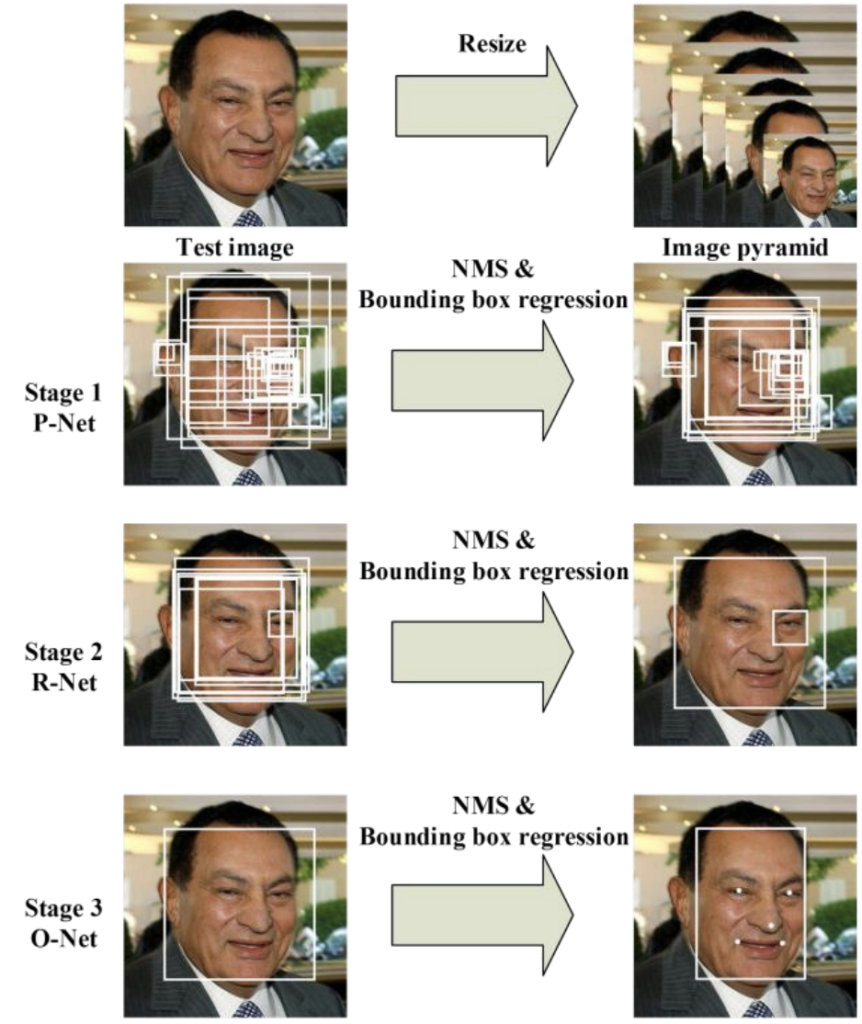
\includegraphics[width=0.7\columnwidth]{images/face-recognition/mtcnn.png}
    \caption{MTCNN face detection pipeline~\cite{MTCNN}.}
    \label{fig:mtcnn}
\end{figure}

Figure~\ref{fig:mtcnn} is a visualization of this three stage process.

\section{Commercial Systems}\label{sec:systems}
There are two main approaches of training CNNs for face recognition.

The first one is to train a multi-class classifier which can separate identities directly.
An example of such system is DeepFace~\ref{subsec:deepface}.

The second approach is to learn embedding using a triplet loss~\ref{sec:triplet-loss} function or similar.
FaceNet~\ref{subsec:facenet} is a known example of a system being trained using the second approach.

\subsection{DeepFace}\label{subsec:deepface}
DeepFace~\cite{DeepFace} is a system developed by FaceBook Inc. in 2014.

The research is notable for its use of advanced alignment technique which consists of three steps:

\begin{enumerate}
    \item The first step is \textbf{2D Alignment} and it begins with detection of 6 fiducial points/landmarks.
    These points and the reference position of points are then used to find a transformation.
    This transformation then generates 2D aligned and cropped image.
    \item The second step is \textbf{3D Alignment}.
    In this step the image is warped onto a generic 3D shape model.
    This is achieved by localization of 67 fiducial points in the image and then fitting an affine
    camera\footnote{linear mathematical model to approximate the perspective projection followed by an ideal
    pinhole camera.} \textit{P} using the generalized least squares solution and the reference position $x_{3d}$ of
    points on the 3D shape model.
    \item \textbf{Frontalization} is the final step and it is achieved by a piece-wise affine transformation T from
    $x_{2d}$ source to $\tilde{x_{3d}}$ target.
    The target $\tilde{x_{3d}}$ is a list of positions of reference fiducial points from previous step enriched with
    residuals \textit{r}.
    These residuals were added to the reference positions $\tilde{x_{3d}}$ to account for non-rigid deformations which
    are not modeled by the affine camera \textit{P}.
    Without these residuals, all faces would be warped into the same shape losing important discriminative factors.
\end{enumerate}

\begin{figure}[H]
    \centering
    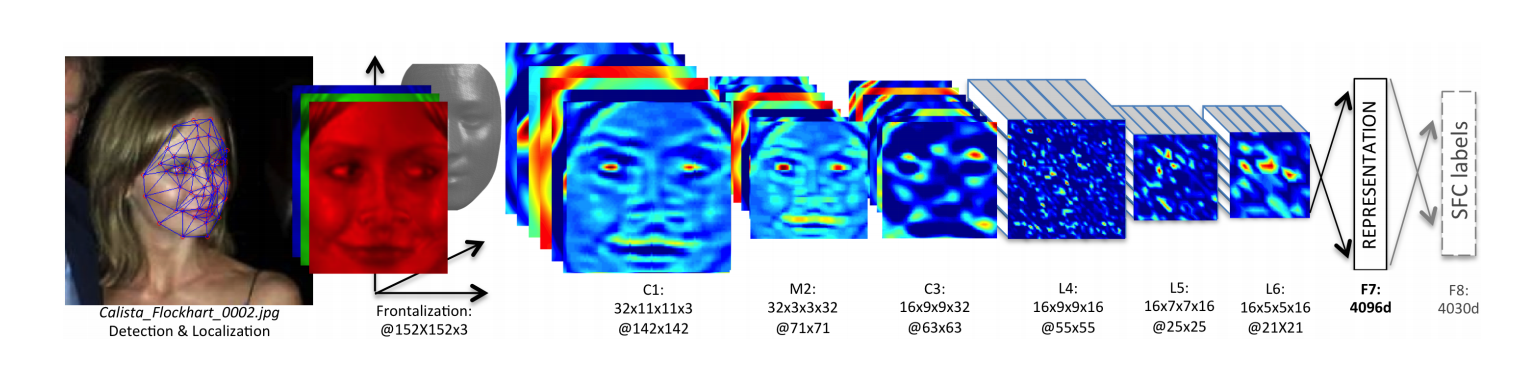
\includegraphics[width=\columnwidth]{images/face-recognition/deepface.png}
    \caption{Outline of DeepFace architecture~\cite{DeepFace}}
    \label{fig:deepface}
\end{figure}

There are 9 layers in the model with over 120 million parameters.
The process of classification is visualized in the picture~\ref{fig:deepface}.
The model was trained on more than 4 million images and as the name of the research paper~\cite{DeepFace} implies,
the results (\textbf{97.35\%} on LFW dataset~\ref{subsec:lfw}) almost matched the results of humans (\textbf{97.53\%}
on LFW dataset).


\subsection{FaceNet}\label{subsec:facenet}
FaceNet~\cite{FaceNet} is a system developed by researchers from Google Inc. in 2015.

Interesting innovation of FaceNet lies in the format of its output.
The output of the network is a vector representing a position in an euclidean space (so called embeddings) instead of a
number representing identity.
This approach allows for straight-forward implementation of \textit{verification} and
\textit{identification}~\ref{ch:face-rec}.
Implementation of verification involves thresholding the distance between two embeddings; and identification becomes
k-NN classification problem.

\begin{figure}[H]
    \centering
    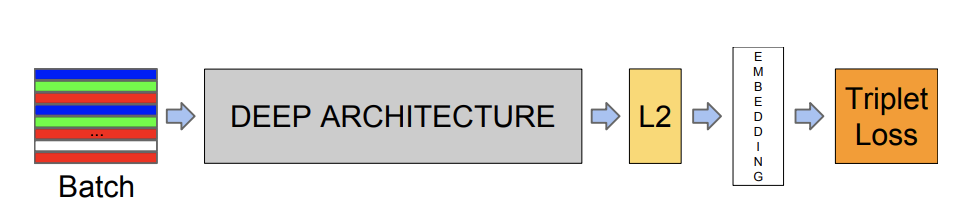
\includegraphics[width=\columnwidth]{images/face-recognition/facenet.png}
    \caption{Outline of FaceNet architecture~\cite{FaceNet}}
    \label{fig:facenet}
\end{figure}

The loss function used to train the model is called \textit{triplet loss}~\ref{sec:triplet-loss}.
Researches at Google came up with new online method\footnote{Training samples are selected during training.} of which
ensures rising difficulty of triplets as the network trains.

The advantages of the model are its accuracy and the compactness of the face representation.
The accuracy of the model exceeded that of human with \textbf{99.63\%} on LFW dataset~\ref{subsec:lfw} and the
euclidean space has only 128 dimensions.
Another advantage is that the model achieved great results on faces which are not in ideal position without using any
of the complex 3D modeling techniques (as was the case in DeepFace system~\ref{subsec:deepface}).
To use proper terms the system is \textit{pose invariant}.